\documentclass[11pt,a4paper]{article}
\usepackage[english,greek]{babel}
\usepackage[utf8]{inputenc}
\usepackage{nimbusserif}
\usepackage[T1]{fontenc}
\usepackage[left=2.00cm, right=2.00cm, top=2.00cm, bottom=2.00cm]{geometry}
\usepackage{amsmath}
\let\myBbbk\Bbbk
\let\Bbbk\relax
\usepackage[amsbb,subscriptcorrection,zswash,mtpcal,mtphrb,mtpfrak]{mtpro2}
\usepackage{siunitx, graphicx,multicol,multirow,enumitem,tabularx,mathimatika,gensymb,venndiagram,hhline,longtable,tkz-euclide,fontawesome5,eurosym,tcolorbox,wrap-rl}
\tcbuselibrary{skins,theorems,breakable}
\newlist{rlist}{enumerate}{3}
\setlist[rlist]{itemsep=0mm,label=\roman*.}
\newlist{alist}{enumerate}{3}
\setlist[alist]{itemsep=0mm,label=\alph*.}
\newlist{balist}{enumerate}{3}
\setlist[balist]{itemsep=0mm,label=\bf\alph*.}
\newlist{Alist}{enumerate}{3}
\setlist[Alist]{itemsep=0mm,label=\Alph*.}
\newlist{bAlist}{enumerate}{3}
\setlist[bAlist]{itemsep=0mm,label=\bf\Alph*.}
\renewcommand{\textstigma}{\textsigma\texttau}
\newlist{thema}{enumerate}{3}
\setlist[thema]{label=\bf\large{ΘΕΜΑ \textcolor{black}{\Alph*}},itemsep=0mm,leftmargin=0cm,itemindent=18mm}
\newlist{erwthma}{enumerate}{3}
\setlist[erwthma]{label=\bf{\large{\textcolor{black}{\Alph{themai}.\arabic*}}},itemsep=0mm,leftmargin=0.8cm}

\newcommand{\lysh}{\textcolor{black}{\textbf{\faCheck\ \ ΛΥΣΗ}}}
\renewcommand{\textstigma}{\textsigma\texttau}
%----------- ΟΡΙΣΜΟΣ------------------
\newcounter{orismos}[section]
\renewcommand{\theorismos}{\thesection.\arabic{orismos}}   
\newcommand{\Orismos}{\refstepcounter{orismos}{\textbf{\textcolor{black}{\kerkissans{Ορισμός\hspace{2mm}\theorismos}}\;:\;}{}}}

\newenvironment{orismos}[1]
{\begin{tcolorbox}[title=\Orismos {\textcolor{black}{\kerkissans{#1}}},breakable,bottomtitle=-1.5mm,
enhanced standard,titlerule=-.2pt,toprule=0pt, rightrule=0pt, bottomrule=0pt,
colback=white,left=2mm,top=1mm,bottom=0mm,
boxrule=0pt,
colframe=white,borderline west={1.5mm}{0pt}{black},leftrule=2mm,sharp corners,coltitle=black]}
{\end{tcolorbox}}

\newcommand{\kerkissans}[1]{{\fontfamily{maksf}\selectfont \textbf{#1}}}
\renewcommand{\textdexiakeraia}{}

\usepackage[
backend=biber,
style=alphabetic,
sorting=ynt
]{biblatex}

\begin{document}
\begin{center}
{\LARGE \kerkissans{Μαθηματικά Γ' ΕΠΑ.Λ}}\\
{\large \kerkissans{Επαναληπτικό διαγώνισμα 1ο Κεφάλαιο\\\today}}
\end{center}
\begin{thema}
\item\mbox{}\\\vspace{-5mm}
\begin{erwthma}
\item Δίνονται συναρτήσεις $f,g$ με πεδία ορισμού $A,Β$ αντίστοιχα και $x_0\in A\cap B$. Να αποδείξετε ότι \[ \left(f(x)+g(x)\right)'=f'(x)+g'(x) \]
\item Να διατυπώσετε το κριτήριο μονοτονίας για μια γνησίως αύξουσα συνάρτηση $f$.
\item Πότε μια συνάρτηση $f$ ονομάζεται συνεχής σε ένα σημείο $x_0$ του πεδίου ορισμού της;
\item Να χαρακτηρίσετε καθεμία από τις παρακάτω προτάσεις ως \textbf{Σωστή} ή \textbf{Λάθος}.
\begin{alist}
\item Ισχύει ότι $ (\sqrt{3})'=\frac{1}{2\sqrt{3}} $.
\item Το πεδίο ορισμού της $ f' $ είναι υποσύνολο του πεδίου ορισμού της $ f $.
\item Αν ισχύει $f'(x_0)=0, f'(x)>0 $ για $x\in(a,x_0)$ και $f'(x)<0$ για $x\in(x_0,\beta)$ τότε η $f$ παρουσιάζει ελάχιστο στη θέση $x_0\in(a,\beta)$.
\item Ισχύει ότι $ \syn{x}=\hm{x} $
\item Ισχύει ότι $ (cf(x))'=cf'(x) $.
\end{alist}
\end{erwthma}
\item Δίνεται η συνάρτηση $f(x)=\dfrac{x^2-a}{x-2}$ για την οποία ισχύει ότι 
\[ \lim_{x\to 2}{\left[f(x)(x^2-4)\right]}=7-a \]
\begin{erwthma}
\item Να αποδείξετε ότι $ a=3 $.
\item Να βρεθεί η εξίσωση της εφαπτομένης της γραφικής παράστασης της $f$ στο σημείο $A(1,f(1))$.
\item Να μελετήσετε τη συνάρτηση $f$ ως προς τη μονοτονία και τα ακρότατα.
\item Να συγκρίνετε τους αριθμούς $f\left(\frac{2023}{2022}\right)$ και $f\left(\frac{2024}{2022}\right)$.
\end{erwthma}
\item
Δίνεται η συνάρτηση $ f(x)=x^2+(a-3)x+a-4 $ της οποίας η γραφική παράσταση διέρχεται από το σημείο $ A(3,4) $.
\begin{erwthma}
\item Να αποδείξετε ότι $ a=2 $.
\item Να δείξετε ότι για κάθε $ x\in\mathbb{R} $ ισχύει
\[ x^2f''(x)-xf'(x)+f(x)=x^2-2 \]
\item Να υπολογίσετε το όριο
\[ \lim_{x\to 2}\frac{\sqrt{f'(x)}-\sqrt{3}}{x-2} \]
\item Βρείτε την τιμή του $x$ για την οποία η συνάρτηση $g(x)=x\cdot f(x)-x^3$ παίρνει μέγιστη τιμή.
\end{erwthma}
\item\mbox{}\\
\wrapr{-5mm}{8}{3cm}{-5mm}{
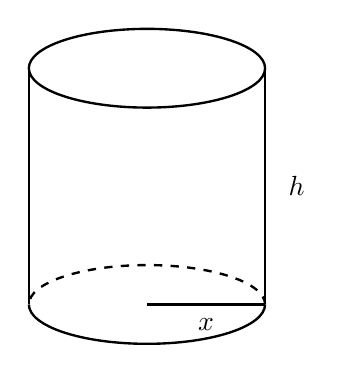
\begin{tikzpicture}
\draw[line width=.3mm] (1.5,.5) ellipse [x radius=1.5,y radius=.5]  ;
\draw[line width=.3mm] (3,-2.5) arc(0:-180:1.5cm and .5cm)  ;
\draw[line width=.3mm,dashed] (3,-2.5) arc(0:180:1.5cm and .5cm)  ;
\draw[line width=.3mm] (3,0.5)--(3,-2.5);
\draw[line width=.3mm] (0,0.5)--(0,-2.5);
\draw[line width=.3mm] (1.5,-2.5)--(3,-2.5);
\node (a) at (3.4,-1) {$ h $};
\node (b) at (2.25,-2.75) {$ x $};
\end{tikzpicture}}{Ενα εργοστάσιο κονσερβοποιίας κατασκευάζει κονσέρβες χωριτικότητας $500\ \mathrm{ml}$ για συμπυκνωμένο γάλα. Ο κύλινδρος έχει ακτίνα βάσης $x\ \mathrm{cm}$ και ύψος $h\ \mathrm{cm}$.
\begin{erwthma}
\item Να δείξετε ότι το ύψος $h$ του κυλίνδρου δίνεται από τη συνάρτηση $h(x)=\frac{500}{\pi x^2}$.
\item Να βρείτε το ρυθμό μεταβολής του εμβαδού το κυλίνδρου όταν το ύψος του ισούται με $h=\frac{20}{\pi}\ \mathrm{cm}$.
\item Να βρεθεί η τιμή του $x$ για την οποία το εμβαδόν της κονσέρβας γίνεται ελάχιστο.
\item Αν το υλικό κατασκευής κοστίζει $12$\euro\  άνα τετραγωνικό μέτρο, να βρεθεί το κόστος κατασκευής μιας κονσέρβας με ελάχιστο εμβαδόν.
\end{erwthma}
(Δίνεται το εμβαδόν του κυλίνδρου $E=2\pi\rho^2+2\pi\rho h$ και ο όγκος του $V=\pi\rho^2 h$.)}
\end{thema}
\end{document}
